\documentclass[12pt,a4paper,british,landscape]{article}

\renewcommand*\ttdefault{cmvtt}
\renewcommand{\familydefault}{\ttdefault}

\usepackage[OT2,T1]{fontenc}

\renewcommand\labelitemi{---}


\usepackage{graphicx}
\usepackage[
    a4paper,
    bindingoffset=0.1cm,
    left=1cm,
    right=1cm,
    top=1.2cm,
    bottom=-1cm,
    footskip=0cm
]{geometry}

\frenchspacing              % Better looking spacings after periods
\pagestyle{empty}           % No pagenumbers/headers/footers



\begin{document}


\begin{figure}[h]
    \vspace{0.15cm}
    \begin{center}
        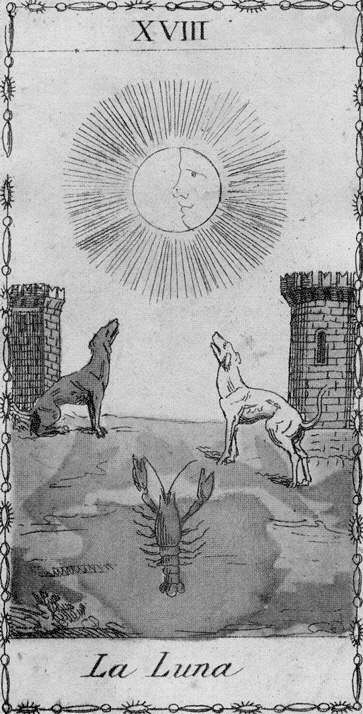
\includegraphics[scale=0.6]{tarot.jpg}
    \end{center}
\end{figure}

\begin{center}
    (ferdinando gumppenberg: lombardy tarot. 1810)
\end{center}

\end{document}

